\subsection{Optimal settings 
for the Cross-entropy method \label{optimalsettingsce}}

In this section we will determine the optimal settings for \begin{changebar}
\cbcolor{blue}
the Cross-entropy method
\end{changebar} through testing
of various adjustable parameters.\\
Compared to CMA-ES, the Cross-entropy method has fewer customizable parameters, more specifically 
only population-parent size and games played per agent.

\subsubsection{Population and selection size}
Other researchers run the Cross-entropy method with population size of
$\populationSize = 100$ and an offspring corresponding to 10\% of 
the population size, resulting in $\offspringNumber = 10$. As it's not 
discussed why this exact setting is applied, various settings of the Cross-entropy method
was executed to asses the performance of other configurations
in our experiments.
The experiments includes different population sizes 
$\populationSize \in \{12, 22, 50, 100, 200\}$ and offspring 
sizes of either $10\%$ and $50\%$ (since the CMA-ES algorithm by default
uses $50 \%$ selected vectors). 
A summary of the experiments can be seen in figure \ref{CEConfigTest}
on page \pageref{CEConfigTest}.

\begin{figure}[H]
\centering
\begin{tabular}{r r | r r r r}
$\populationSize$ & $\offspringNumber$ & mean & Q1 & Q2 & Q3\\
\hline
13 & $10\%$  & 1585,3     & 93,0      & 113,5        & 220,7\\
13 & $25\%$  & 30.496,9   & 15.222,1  & 20.264,2     & 39.019,8\\
13 & $50\%$  & 39.824,2   & 26.457,0  & 33.663,4     & 49.743,7\\
22 & $10\%$  & 35.841,6   & 20.391,9  & 42.045,5     & 48.464,6\\
22 & $25\%$  & 80.884,9   & 56.042,5  & 71.900,2     & 78.653,4\\
22 & $50\%$  & 52.887,4   & 23.531,9  & 42.161,0     & 83.144,1\\
50 & $10\%$  & 95,623,1   & 82.738,9  & 93.388,9     & 111.351,5\\
50 & $25\%$  & 110.525,0  & 103.128,1 & 111.195,5    & 121.974,4\\
50 & $50\%$  & 69.130,7   & 52.511,0  & 64.351,6     & 91.488,6\\
\hdashline
100 & $10\%$ & 115.868,7  & 84.368,5  & 122.238,5    & 146.457,0\\
\hdashline
100 & $25\%$ & 70.011,1   & 58.008,0  & 69.588,2     & 80.432,7\\
100 & $50\%$ & 22.910,4   & 4.037,7   & 14.353,7     & 47.215,9\\
200 & $10\%$ & 85.181,7   & 45.201,5  & 96.803,1     & 117.578,0\\
200 & $25\%$ & 32.894,6   & 8688,7    & 25.333,1     & 58.434,8\\
200 & $50\%$ & 946,4      & 585,0     & 802,5        & 1.267,7
\end{tabular}
\caption{the Cross-entropy method configuration test, 
see Appendix \ref{appendixCrossEntropyConfig} for the full plots 
of the experiments.  \label{CEConfigTest}}
\end{figure}

The experiments with different population and parent sizes
does not seem to support a choice for any other configuration 
than the mostly commonly used 
$\populationSize = 100$ and $\offspringNumber = 10$. \\
However, with a configuration of $\populationSize = 50$ and $\offspringNumber = 12$ convergence
is achieved faster (see figure \ref{fig:bestConfCE}). This means that the score limit is reached faster, which
results in longer computation time, than the $\populationSize = 100$ and $\offspringNumber = 10$
configuration. In other words, the $\populationSize = 100$ and $\offspringNumber = 10$ configuration 
is therefore preferred since it takes shorter computation time and the end-result is similar compared
to the $\populationSize = 50$ and $\offspringNumber = 12$ configuration, even though the latter 
configuration from our expriments converged faster. The experiments also apppears
to suffer from a high noise, yet both the mean and the quantiles favor the 
extensively tested the Cross-entropy method configuration of $\populationSize = 100$ and $\offspringNumber = 10$.

\begin{changebar}
\cbcolor{blue}
\begin{figure}[H]
\begin{tabular}{@{}l@{}l@{}}
\includegraphics[scale=1]{plots/ce_ConstantNoise_l50_o12_all} &
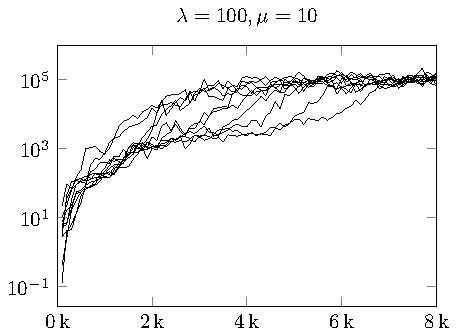
\includegraphics[scale=1]{plots/ce_ConstantNoise_l100_o10_all}
\end{tabular}
\caption{The two best configurations of the Cross-entropy method 
\label{fig:bestConfCE}}
\end{figure}
\end{changebar}

\subsubsection{Games per agent \label{GamesPerAgentCESection}}
Another parameter we can adjust is the number of 
games played each agent plays per generation. By playing
multiple games with each agent and using their 
mean score to compute the next generation mean. This
secures a higher chance of a better offspring generation,
but at the cost of more games
evaluated.\\
Table \ref{GamesPerAgentCE} shows the different values of
games per agent we are going to be
testing.

\begin{table}[H]
\centering
\begin{tabular}{c c c}
Population Size & Parent size & Games per Agent\\
\hline
$13$ & $10\%$ & 1/3/5/7/10\\
$13$ & $25\%$ & 1/3/5/7/10\\
$13$ & $50\%$ & 1/3/5/7/10\\
$22$ & $10\%$ & 1/3/5/7/10\\
$22$ & $25\%$ & 1/3/5/7/10\\
$22$ & $50\%$ & 1/3/5/7/10\\
$50$ & $10\%$ & 1/3/5/7/10\\
$50$ & $25\%$ & 1/3/5/7/10\\
$50$ & $50\%$ & 1/3/5/7/10\\
$100$ & $10\%$  & 1/3/5/7/10\\
$100$ & $25\%$  & 1/3/5/7/10\\
$100$ & $50\%$ & 1/3/5/7/10\\
$200$ & $10\%$ & 1/3/5/7/10\\
$200$ & $25\%$ & 1/3/5/7/10\\
$200$ & $50\%$ & 1/3/5/7/10
\end{tabular}
\caption{Games per agent of the Cross-entropy method experiment setup\label{GamesPerAgentCE}}
\end{table}

The experiments includes different games per agent of $\{1,3,5,7,10\}$. By increasing the number of games 
played per agent, we are increasing the evaluation cost by a multiplication factor in exchange for a more 
accurate evaluation of each agent. This is to avoid misconceiving poor performing agents
for good ones, as multiple evaluations will decrease the chance the agent having 
'lucky games'. However, we wish to find 
the best performing configuration with the lowest cost and maximum benefit, and evaluating multiple 
times will increase the function cost.\\
\\
\textbf{Results}\\
The total number of configuration experiments is 75, with 30 individual experiments each,
resulting in a total of
\begin{changebar} 
2,250
\end{changebar} 
individual experiment runs. These results are all included in 
appendix \ref{appendixCEPopulationParent}.\\
Below in table \ref{CEBestConfigTable} and figure \ref{CEBestConfigPlot}, the five best
best resulting configurations are depicted. We chose these by first selecting the best 
configuration of each Population-Parent size. This resulted in three
configurations for each Population-Parent size, which we then compared to determine the best
configuration for each Population-Parent size. Which is depicted in table \ref{CEBestConfigTable} and figure \ref{CEBestConfigPlot}.
\begin{table}[H]
\centering
\small
\begin{tabular}{r r r r r r r}
Population & Parent & Games per Agent & mean & Q1 & Q2 & Q3\\
\hline
$12$ & $6$ & 10 & $2109.837$ & $1802.968$ & $2021.165$ & $2276.652$\\
$22$ & $5$ & 5 & $2371.793$ & $2013.168$ & $2412.815$ & $2708.931$\\
$50$ & $12$ & 5 & $2749.991$ & $2605.171$ & $2702.400$ & $2835.960$\\
$100$ & $25$ & 3 & $2776.560$ & $2397.691$ & $2742.950$ & $3027.541$\\
$200$ & $50$ & 1 & $2950.767$ & $2564.118$ & $2841.065$ & $3377.189$\\
\end{tabular}
\caption{Best configurations of all population sizes - the Cross-entropy method \label{CEBestConfigTable}}
\end{table}

\begin{figure}[H]
\centering
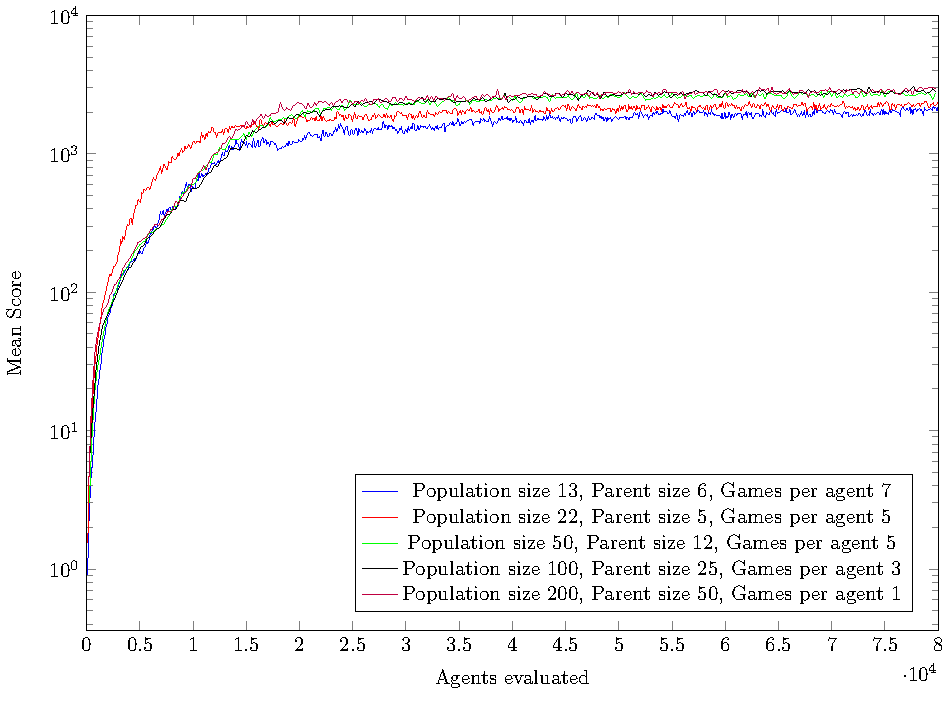
\includegraphics[scale=0.8]{data/ce_population_offspring/bestofall_population/PlotFile.pdf}
\caption{Best configurations of all population sizes - the Cross-entropy method \label{CEBestConfigPlot}}
\end{figure}

From table \ref{CEBestConfigTable} and figure \ref{CEBestConfigPlot}, we can see that population size 50 with parent size 12 and 5 games per agent, population size 100 with parent size 25 and 3 games per agent, and, population size 200 with parent size 50 and 1 game per agent, performs almost identically.\\

\textbf{Discussion and analysis}\\
From the graph and the table depicting the quantiles, it appears that the configuration
population size 200 with parent size 50 and 1 game per agent yields the best performance. 
It achieves the highest score with the fastest convergence of all the candidate solutions
we have listed.\\
Therefore, we will be using this configuration for the tuned comparison experiments.
